\chapter{Vorbereitung}
Supraleiter zeichnen sich durch eine widerstandslose Leitung unter einer kritischen
Temperatur $T_c$ aus. Schon seit Anfang des 20. Jahrhunderts bekannt ist dies in
Metallen bei sehr tiefen Temperaturen nahe des Nullpunktes. Hochtemperatursupraleiter
konnten dagegen erst 1986 entdeckt werden. Die theoretischen Grundlagen hinter 
diesen Effekten sind zahlreich und zum Teil noch heute ungeklärt. Hier soll ein
kleiner Überblick gegeben werden.

	\section{Theoretische Grundlagen}

    \subsection{Bosonen und Fermionen}
Zum Verständnis der Supraleitung essentiell ist die Unterscheidung der 
Elementarteilchen in Bosonen und Fermionen, sowie die Eigenschaften Dieser.
Für unsere Zwecke genügt es Bosonen und Fermionen zu betrachten.

        \subsubsection{Fermionen}
Als Fermionen werden Teilchen mit halbzahligem Spin ($\frac{1}{2}, \frac{3}{2},
\dots$) bezeichnet. Diese Gruppe der Elementarteilchen, zu der Quarks und 
Leptonen gezählt werden, bildet die Materie.
\vspace{3pt}\\
Für die Supraleitung wichtig ist vor allem das Pauli'sche Ausschlussprinzip, 
welchem Fermionen unterliegen. Es besagt, dass 2 Fermionen am selben Ort nicht
den selben Quantenzustand besetzen dürfen.\\
Dies wird am Beispiel der Elektronen in Atomorbitalen klar. Ohne dieses Prinzip
könnten alle Elektronen im energetisch günstigsten Grundzustand liegen, in Atomen
werden jedoch Besetzungen energetisch höherliegender Zustände beobachtet.
\begin{figure}[h]
    \centering
    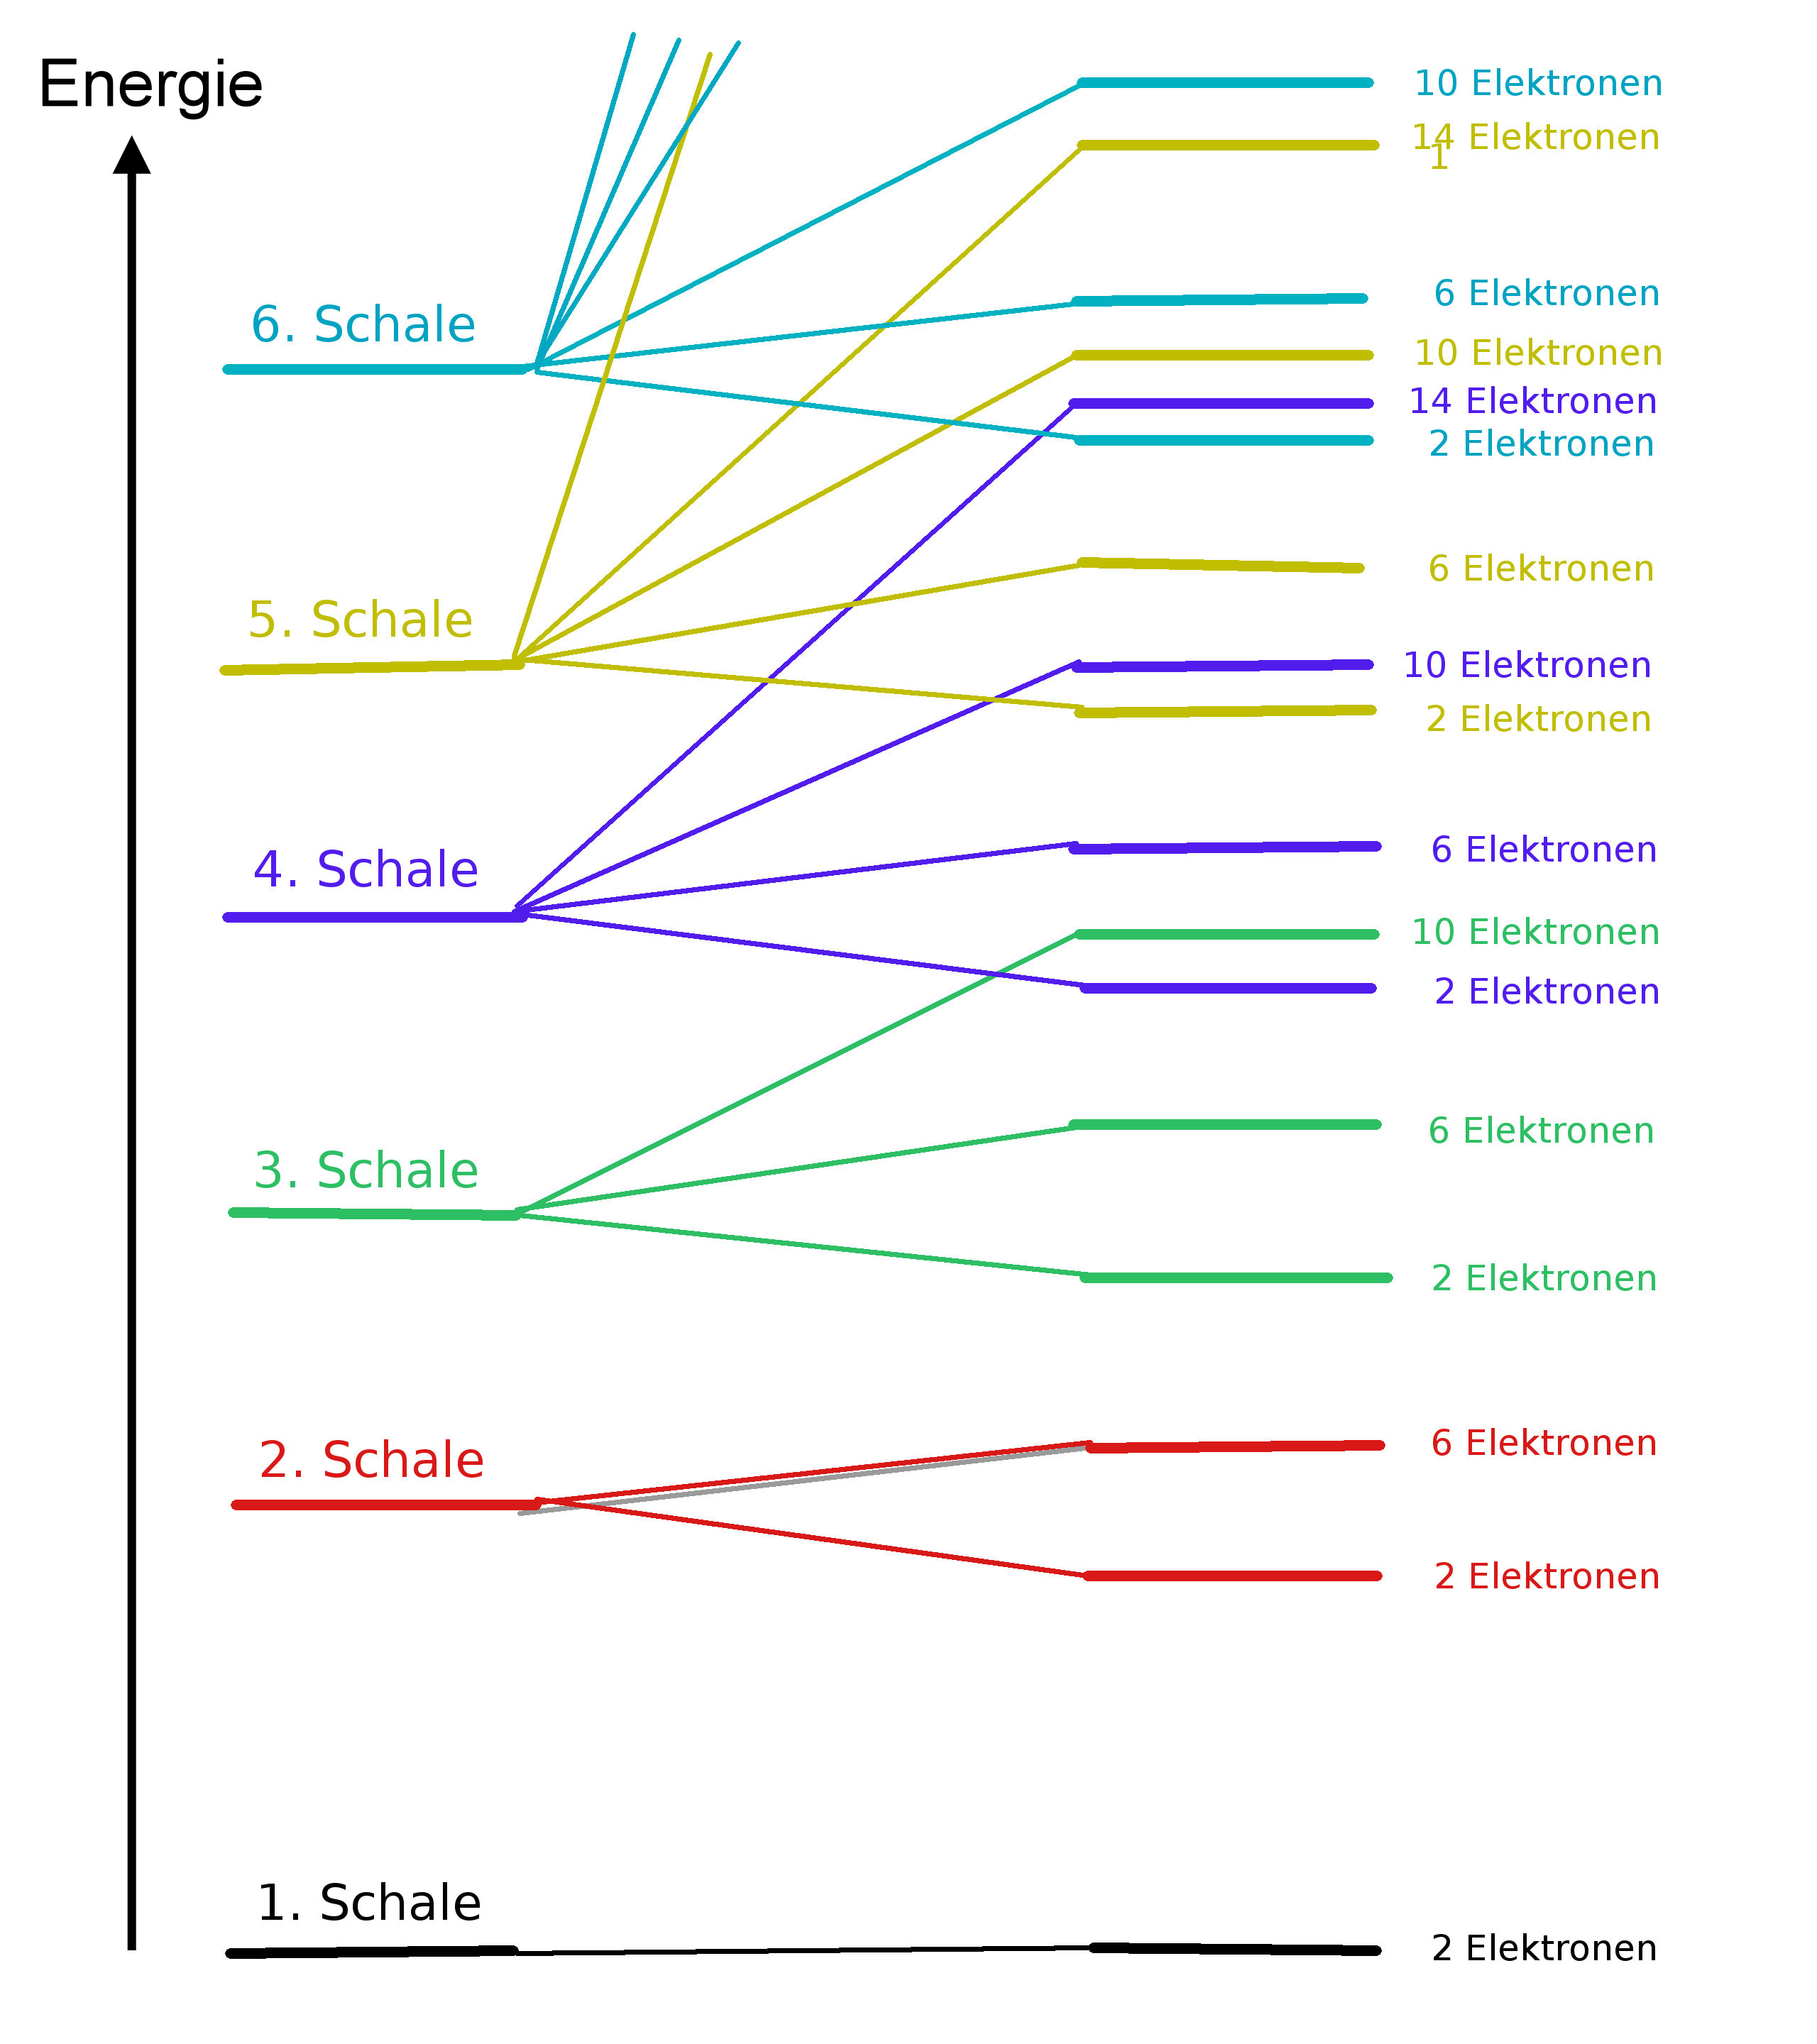
\includegraphics[width=0.4\textwidth]{Abb/energieniveaus-elektronen.jpg}
    \caption{Energieniveaus der Elektronen in Atomorbitalen [1]}
    \label{Abb:energieschema}
\end{figure}
In Abbildung \ref{Abb:energieschema} ist die Aufteilung zu sehen. Zuerst werden die
beiden Zustände der ersten Schale besetzt, die sich nur in der Spinausrichtung 
unterscheiden. In den nächsten Schalen werden durch unterschiedliche Drehimpulse 
und Spinausrichtungen der einzelnen Elektronen weitere Zustände besetzt, mit immer
größer werdender Energie.

        \subsubsection{Bosonen}
Als Bosonen werden Teilchen mit ganzzahligem Spin bezeichnet. Elementar treten 
Bosonen nur als Austauschteilchen der elementaren Wechselwirkungen zwischen 
Fermionen auf. Ein Beispiel ist hier das Photon als Überträger der 
elektromagnetischen Kraft. Für unsere Zwecke sind jedoch aus Fermionen
zusammengesetzte Bosonen weitaus wichtiger.
\vspace{3pt}\\
Mehrere Fermionen können durch Wechselwirkungen so aneinander koppeln, dass sie
durch eine gemeinsame Gesamtwellenfunktion beschrieben werden müssen. Einfach
hat dies zur Folge, dass sich Verbunde aus Fermionen, ein bekanntes Beispiel 
hierfür stellen Atomkerne dar, wie Bosonen verhalten. 
\vspace{3pt}\\
Im Gegensatz zu den Fermionen unterliegen Bosonen nicht dem Pauli-Prinzip. Anders
als im obigen Energieschema, ist es also für Bosonen möglich den selben
Energiezustand zu besetzen. Dies wird später für die Theorie der Supraleitung 
essentiell.
   
	\subsection{BCS-Theorie}
Eine gute theoretische Beschreibung Supraleiter 1. Art bietet die BCS-Theorie. 
Zwar kann durch diese die Hochtemperatursupraleitung auch erklärt werden, das 
Prinzip der Paarbildung bleibt jedoch ungeklärt.

        \subsubsection{Cooper-Paare}
Grundlage der Supraleitung ist die Cooper-Paarbildung der Elektronen im Festkörper.
\vspace{3pt}\\
Es wird angenommen, dass ein Elektron, aufgrund seiner negativen Ladung, eine 
Deformationsspur hinterlässt. 
\begin{figure}[h]
    \centering
    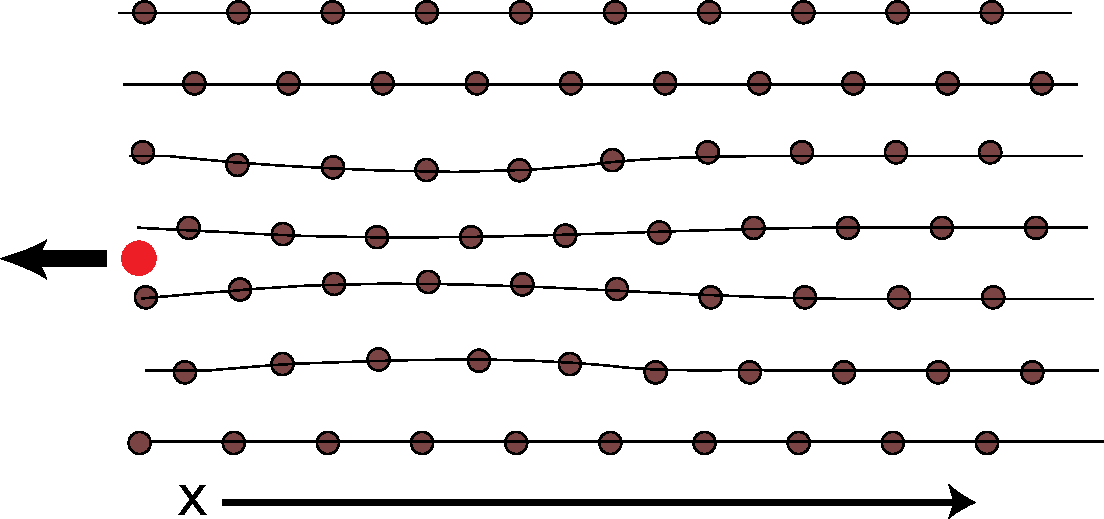
\includegraphics[width=0.7\textwidth]{Abb/deformation.pdf}
    \caption{Deformationsspur hinter einem Elektron}
    \label{Abb:def}
\end{figure}
Siehe hierzu Abbildung \ref{Abb:def}. Ein Elektron zieht die positiv geladenen Kerne
an, was diese zum Schwingen anregt. Nach einer viertel Schwingperiode erreicht die
Konzentration der positiven Ladungen ihr Maximum und weitere Elektronen werden 
angezogen. Durch die große Reichweite dieser Kraft, das erste Elektron ist nach
einer viertel Schwingperiode schon weit durch den Festkörper gewandert, wird sie
nicht durch die Coulomb-Abstoßung aufgehoben.
\vspace{3pt}\\
Grundlage der BCS-Theorie ist nun die Kopplung zweier Elektronen durch diese 
Wechselwirkung, wodurch der Verbund durch eine bosonische Gesamtwellenfunktion
beschrieben werden muss.

    \subsection{Einteilung von Supraleitern}
Wie bereits erwähnt gibt es verschiedene Arten von Supraleitern, die Typ-I und
Typ-II Supraleiter. Unterschieden wird hier anhand des Verhaltens in einem 
Magnetfeld. 

        \subsubsection{Typ-I Supraleiter}
Der Typ-I Supraleiter ist der "klassische" Supraleiter. Die meisten Metallischen
können hier zugeordnet werden. Legt man an einen Typ-I Supraleiter im 
normalleitenden Zustand ein Magnetfeld an und kühlt diesen anschließend auf
$T<T_c$, so wird das innere Magnetfeld, bis auf einen kleinen Bereich am Rand,
vollständig verdrängt. Die supraleitende Phase kann durch ein Erwärmen über die
kritische Temperatur $T_c$, das Anlegenen eines starken Magnetfelds mit einer 
Feldstärke größer der kritischen Feldstärke $B_c$, oder dem Überschreiten
der kritischen Stromdichte $J_c$ durchbrochen werden.\\
Weiter haben Materialien diesen Typs meist eine sehr niedrige Sprungtemperatur 
$T_c$ von nur wenigen Kelvin.

        \subsubsection{Typ-II Supraleiter}
Der Typ-II Supraleiter zeigt bis zum unteren kritischen Magnetfeld $B_{c1}$ 
dasselbe Verhalten. Wird ein stärkeres Magnetfeld angelegt, so können Feldlinien
in Form von Flussschläuchen (extra Kapitel?) in das Material eindringen. Durch
ein Wandern dieser Flussschläuche und der daraus resultierenden Feldbewegung,
entsteht auch ein elektrischer Widerstand im Supraleiter.

%\begin{itemize}
%    \item Bosonische Gesamtwellenfunktion
%    \item Stöße durch Energiezustand nicht möglich?
%    \item bosonen und fermionen
%\end{itemize}
